\documentclass{article}
\usepackage{titlesec}
\titleclass{\subsubsubsection}{straight}[	hesubsubsection]
\newcounter{subsubsubsection}[subsubsection]
\renewcommand\thesubsubsubsection{\thesubsubsection.\arabic{subsubsubsection}}
\titleformat{\subsubsubsection}{\normalfont\normalsize\bfseries}{\thesubsubsubsection}{1em}{}
\titlespacing*{\subsubsubsection}{0pt}{1.5ex plus .1ex}{0.5ex plus .1ex}
\usepackage{graphicx}
\usepackage{fancyhdr}

\pagestyle{fancy}
\fancyhf{}
\fancyhead[L]{Alireza Haghighi}
\fancyhead[R]{CW-Final Assignment}
\fancyfoot[C]{\thepage}

\title{Final Assignment}
\author{Alireza Haghighi}
\date{\today}

\begin{document}

\begin{titlepage}
    \maketitle
    \thispagestyle{empty}
\end{titlepage}

\newpage
\tableofcontents
\thispagestyle{empty}

\newpage

\section{Git and GitHub}
\subsection{Repository Initialization and Commits}
At first, I opened GitHub and signed in to my account. Then I went to my repository and clicked on the NEW button. Then I wrote the name of my repository and made it public. Then I clicked on the OK button to make that repository.

\subsection{GitHub Actions for LaTeX Compilation}
At first I had a weird problem with creating ".github/workflows" directory. So I created the directory and "main.yml" in the meantime. It worked and I copied the code for this file and used it for my LaTeX file.

\section{Exploration Tasks}
\subsection{Vim Advanced Features}
\subsubsection{Global Commands (\texttt{:g})}
The \texttt{:g} command performs operations on lines matching a pattern.

\begin{itemize}
    \item \textbf{Syntax:}
    \begin{verbatim}
    :g/pattern/command
    \end{verbatim}

    \item \textbf{Examples:}
    \begin{itemize}
        \item Delete lines with \texttt{error}:
        \begin{verbatim}
        :g/error/d
        \end{verbatim}

        \item Add a semicolon to lines with \texttt{function}:
        \begin{verbatim}
        :g/function/norm A;
        \end{verbatim}

        \item Copy lines with \texttt{TODO} to the end:
        \begin{verbatim}
        :g/TODO/t$
        \end{verbatim}
    \end{itemize}

    \item \textbf{Inverse Matching (\texttt{:v}):}
    \begin{verbatim}
    :v/error/d
    \end{verbatim}
\end{itemize}

\subsubsection{Advanced Search and Replace}
Vim supports flexible search and replace with regex.

\begin{itemize}
    \item \textbf{Basic Replace:}
    \begin{verbatim}
    :s/old/new/g
    \end{verbatim}

    \item \textbf{Replace in Entire File:}
    \begin{verbatim}
    :%s/old/new/g
    \end{verbatim}

    \item \textbf{Confirm Replacements:}
    \begin{verbatim}
    :%s/old/new/gc
    \end{verbatim}

    \item \textbf{Regex Examples:}
    \begin{itemize}
        \item Replace \texttt{foo} followed by digits:
        \begin{verbatim}
        :%s/foo\d\+/bar/g
        \end{verbatim}

        \item Swap two words:
        \begin{verbatim}
        :%s/\(\w\+\) \(\w\+\)/\2 \1/g
        \end{verbatim}
    \end{itemize}
\end{itemize}

\subsubsection{Text Objects}
Text objects let you operate on blocks of text.

\begin{itemize}
    \item \textbf{Common Text Objects:}
    \begin{itemize}
        \item \texttt{iw} - Inner word
        \item \texttt{aw} - A word
        \item \texttt{i"} - Inside quotes
        \item \texttt{a"} - Around quotes
        \item \texttt{i(} - Inside parentheses
        \item \texttt{a(} - Around parentheses
    \end{itemize}

    \item \textbf{Examples:}
    \begin{itemize}
        \item Delete a word: \texttt{diw}
        \item Change inside quotes: \texttt{ci"}
        \item Yank inside parentheses: \texttt{yi(}
        \item Select a paragraph: \texttt{vip}
    \end{itemize}
\end{itemize}

\subsection{Memory Profiling}
\subsubsection{Memory Leak}
A \textbf{memory leak} occurs when a program allocates memory but fails to release it after it is no longer needed. This leads to a gradual increase in memory usage over time. Memory leaks can happen due to:

\begin{itemize}
  \item \textbf{Unfreed Allocations}: Dynamically allocated memory (e.g., using \texttt{malloc} or \texttt{new}) is not freed (e.g., using \texttt{free} or \texttt{delete}).
  \item \textbf{Lost References}: Pointers to allocated memory are overwritten or go out of scope without freeing the memory.
  \item \textbf{Cyclic References}: In languages with garbage collection, objects reference each other in a cycle, preventing their cleanup.
  \item \textbf{Improper Resource Management}: Failing to close file handles, database connections, or other resources that consume memory.
\end{itemize}

Memory leaks can cause programs to slow down, crash, or exhaust system memory, especially in long-running applications.

\subsubsection{Memory Profilers}
\textbf{Valgrind} is a powerful programming tool used primarily for debugging and profiling applications, especially in C and C++. Its main purpose is to help developers detect memory-related issues, such as memory leaks, invalid memory access, and improper use of dynamically allocated memory. Valgrind achieves this by simulating the execution of a program and tracking all memory operations.

\subsubsubsection*{Key Features of Valgrind:}
\begin{itemize}
  \item \textbf{Memory Leak Detection}:
    \begin{itemize}
      \item Valgrind identifies memory that was allocated but not freed, helping developers locate the source of memory leaks.
      \item It provides detailed reports, including the exact lines of code where the memory was allocated and where it was lost.
    \end{itemize}
  \item \textbf{Invalid Memory Access Detection}:
    \begin{itemize}
      \item It detects issues like reading or writing to memory that has already been freed, accessing memory out of bounds, or using uninitialized memory.
    \end{itemize}
  \item \textbf{Performance Profiling}:
    \begin{itemize}
      \item Valgrind includes tools like Callgrind and Cachegrind to analyze program performance, identifying bottlenecks and inefficient code.
    \end{itemize}
  \item \textbf{Thread Error Detection}:
    \begin{itemize}
      \item It can detect race conditions and improper synchronization in multi-threaded programs.
    \end{itemize}
\end{itemize}

\subsubsubsection*{How Valgrind Helps with Memory Leaks:}
\begin{itemize}
  \item \textbf{Detailed Reports}: When a program is run under Valgrind, it monitors all memory allocations and deallocations. If memory is not freed, Valgrind generates a report showing where the memory was allocated and where it was lost.
  \item \textbf{Error Prevention}: By identifying memory leaks early in the development process, Valgrind helps prevent crashes and performance degradation in production environments.
  \item \textbf{Ease of Use}: Valgrind is easy to integrate into the development workflow. Developers simply run their program with Valgrind (e.g., \texttt{valgrind --leak-check=full ./my\_program}) to get insights into memory usage.
\end{itemize}

\subsubsubsection*{Example Usage:}
\begin{verbatim}
valgrind --leak-check=full ./my_program
\end{verbatim}
This command runs the program \texttt{my\_program} under Valgrind and performs a full memory leak check. The output will show any memory leaks, along with the exact lines of code responsible.

\subsubsubsection*{Benefits:}
\begin{itemize}
  \item Improves program reliability by catching memory-related bugs.
  \item Reduces debugging time by pinpointing the source of memory issues.
  \item Enhances performance by identifying inefficient memory usage.
\end{itemize}

In summary, Valgrind is an essential tool for developers working with low-level languages like C and C++. It helps ensure that programs are free from memory leaks and other memory-related errors, leading to more stable and efficient software.

\subsection{GNU/Linux Bash Scripting}
\subsubsection{fzf}
\subsubsubsection*{What is \texttt{fzf}?}

\texttt{fzf} (fuzzy finder) is a command-line tool that provides fast and intuitive fuzzy searching capabilities. It allows users to interactively search through lists of items (e.g., files, commands, history) by typing partial or mismatched queries. \texttt{fzf} is highly customizable and integrates seamlessly with other CLI tools and workflows.

\subsubsubsection*{What is Fuzzy Searching?}

Fuzzy searching is a technique for finding items that approximately match a given query, even if the query contains typos, missing characters, or is not an exact match. Instead of requiring an exact or prefix match, fuzzy searching ranks results based on how closely they align with the query. For example:

\begin{itemize}
    \item Query: \texttt{abc}
    \item Matches: \texttt{a\_b\_c}, \texttt{axbxc}, \texttt{abracadabra}, \texttt{abc123}
\end{itemize}

Fuzzy searching is particularly useful when you don't remember the exact term or want to quickly narrow down a large list of possibilities.

\subsubsubsection*{Key Features of \texttt{fzf}:}

\begin{itemize}
    \item \textbf{Interactive Search}: Results update in real-time as you type.
    \item \textbf{Fuzzy Matching}: Finds items even with incomplete or misspelled queries.
    \item \textbf{Integration}: Works with tools like \texttt{vim}, \texttt{tmux}, \texttt{zsh}, and more.
    \item \textbf{Customizable}: Supports custom key bindings, previews, and sorting.
    \item \textbf{Fast}: Optimized for performance, even with large datasets.
\end{itemize}
\subsubsubsection*{Description of the Command: \texttt{ls | fzf}}

The command \texttt{ls | fzf} does the following:

\begin{itemize}
    \item \texttt{ls}: Lists the files and directories in the current working directory.
    \item \texttt{|} (Pipe): Takes the output of the \texttt{ls} command and passes it as input to the next command (\texttt{fzf}).
    \item \texttt{fzf}: Opens an interactive fuzzy finder interface where you can search through the list of files and directories. As you type, \texttt{fzf} filters the list in real-time, showing only the items that match your query.
\end{itemize}

\subsubsubsection*{How It Works:}
\begin{itemize}
    \item When you run \texttt{ls | fzf}, the list of files and directories is displayed in the \texttt{fzf} interface.
    \item You can start typing a partial or fuzzy query (e.g., \texttt{doc} to match \texttt{Documents} or \texttt{abc} to match \texttt{a\_b\_c}).
    \item \texttt{fzf} dynamically filters the list, highlighting the best matches.
    \item Once you select an item (by pressing \texttt{Enter}), the selected item is printed to the terminal.
\end{itemize}
\subsubsection{Using fzf to find your favorite PDF}
\subsubsubsection*{List All PDF Files in a Directory}

To list all files with the \texttt{.pdf} extension, you can use the \texttt{fd} command. \texttt{fd} is a fast and user-friendly alternative to \texttt{find} that is designed for simplicity and speed.

\textbf{Command:}
\begin{verbatim}
fd -e pdf
\end{verbatim}

\begin{itemize}
    \item \texttt{fd}: The command to search for files and directories.
    \item \texttt{-e pdf}: Filters the results to only include files with the \texttt{.pdf} extension.
\end{itemize}

This command will recursively search the current directory (and its subdirectories) for all \texttt{.pdf} files and display their paths.

\subsubsubsection*{Select a PDF Using \texttt{fzf}}

Once you have the list of PDF files, you can pipe the output to \texttt{fzf} to interactively select the desired PDF.

\textbf{Command:}
\begin{verbatim}
fd -e pdf | fzf
\end{verbatim}

\begin{itemize}
    \item \texttt{fd -e pdf}: Lists all \texttt{.pdf} files.
    \item \texttt{|}: Pipes the output of \texttt{fd} to \texttt{fzf}.
    \item \texttt{fzf}: Opens an interactive fuzzy finder interface where you can search and select the desired PDF.
\end{itemize}

\subsubsubsection*{How It Works:}
\begin{itemize}
    \item Run \texttt{fd -e pdf | fzf}.
    \item \texttt{fd} will list all \texttt{.pdf} files in the directory and its subdirectories.
    \item The list of PDFs will be passed to \texttt{fzf}, which will display them in an interactive interface.
    \item Start typing part of the PDF name (e.g., \texttt{math} to match \texttt{math\_notes.pdf}).
    \item \texttt{fzf} will dynamically filter the list based on your input.
    \item Press \texttt{Enter} to select the PDF. The selected file's path will be printed to the terminal.
\end{itemize}

\subsubsection{Opening the file using Zathura}

To open the selected PDF file using Zathura, you can combine the \texttt{fd}, \texttt{fzf}, and \texttt{zathura} commands. Here's the command and an explanation of how it works:

\subsubsubsection*{Command to Open the Selected PDF with Zathura:}
\begin{verbatim}
zathura "$(fd -e pdf | fzf)"
\end{verbatim}

\subsubsubsection*{Explanation of the Command:}

\begin{itemize}
    \item \texttt{fd -e pdf}:
    \begin{itemize}
        \item Lists all files with the \texttt{.pdf} extension in the current directory and its subdirectories.
    \end{itemize}
    
    \item \texttt{| fzf}:
    \begin{itemize}
        \item Pipes the list of PDF files to \texttt{fzf}, which allows you to interactively select one file.
    \end{itemize}
    
    \item \texttt{\$(...)}:
    \begin{itemize}
        \item This is called \textbf{command substitution}. It runs the command inside the parentheses (\texttt{fd -e pdf | fzf}) and substitutes the output (the selected file path) into the outer command.
    \end{itemize}
    
    \item \texttt{zathura "\$(fd -e pdf | fzf)"}:
    \begin{itemize}
        \item The selected file path is passed to \texttt{zathura}, which opens the PDF file.
    \end{itemize}
\end{itemize}

\subsubsubsection*{How It Works:}
\begin{itemize}
    \item Run the command:
    \begin{verbatim}
    zathura "$(fd -e pdf | fzf)"
    \end{verbatim}
    \item \texttt{fd} lists all \texttt{.pdf} files.
    \item \texttt{fzf} displays the list of PDFs in an interactive interface.
    \item You type part of the PDF name to filter the list.
    \item Press \texttt{Enter} to select the PDF.
    \item \texttt{zathura} opens the selected PDF file.
\end{itemize}

\section{Git and FOSS}
\subsection{README.md}
I've Included a basic README.md file in my GitHub.

\newpage
\subsection{Issues}
\begin{figure}[htbp]
    \centering
    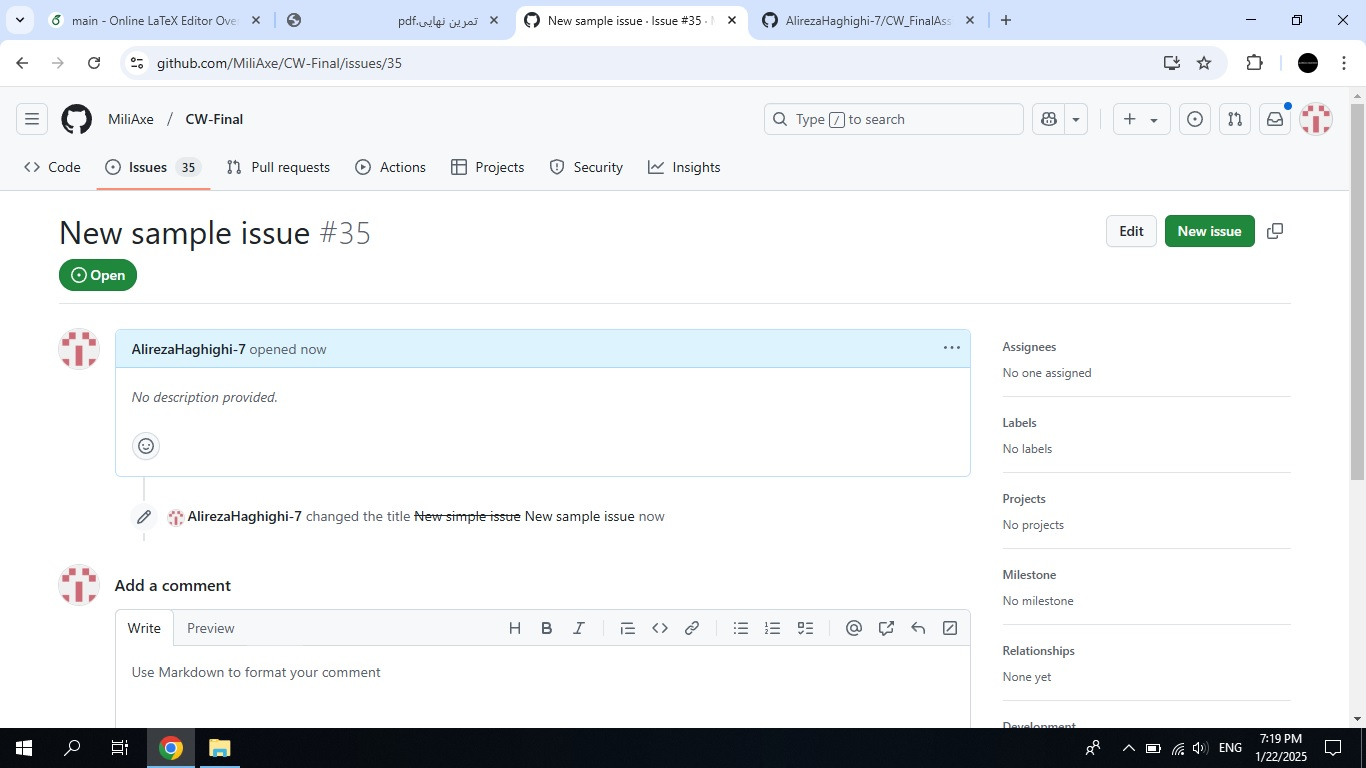
\includegraphics[width=1.3\textwidth]{Untitled.jpg}
    \caption{This is a sample issue.}
\end{figure}

\subsection{FOSS Contribution}
I don't really like FOSS projects because absolutely everyone can participate in it. I'm not really into working with a lot of peple in the meantime so I won't  contribute in a FOSS project.

\end{document}